\chapter{Balance de carga en SPS}
\label{cap:estadoDelArte}

\section{Perspectivas de balance de carga}
\label{sec:perspectivasBC}
Dentro de la literatura se ha observado de distintas perspectivas el problema de balance de carga en un SPS, las cuales consideran los recursos físicos como fuente del problema, y otro enfoque que considera los recursos lógicos como el foco del mismo.

\subsection{Recursos físicos}
\label{subsec:recFisicosBC}
En esta perspectiva se toma en consideración la sobrecarga del sistema dado las limitantes físicas de éste, ya sea por condiciones de los recursos disponibles o por el ambiente de desarrollo. Las estrategias de balance de carga que se presentan están basados en el concepto de umbrales de recursos, es decir, cunado estos umbrales son alcanzados se aplica una estrategia para aliviar la carga. Estos umbrales pueden ser el nivel \textit{Service Level Objective} (SLO) \citep{sturm2000foundations}, porcentaje de CPU utilizada o disponibilidad de la memoria \citep{Dong06schedulingalgorithms}, entre otros.

Una de las soluciones con la perspectiva anterior es Borealis \citep{XingZH05}. Borealis considera la cantidad de carga de los nodos en ventanas de tiempo pre-determinadas, las cuales son monitoreados por un coordinador centralizado. Este coordinador se encarga de analizar los recursos del sistema, y en caso que se sobrepase el umbral propuesto, se aplica la migración de los operadores del nodo hacia a otro nodo candidato cuya carga es menor.

Esta estrategia no soluciona el problema de rendimiento del sistema, debido a que sólo mueve el problema de una máquina a otra. Para elegir al nodo candidato, se realiza un análisis de correlación que existe entre el operador y el nodo candidato, de esta manera, no necesariamente va a ser enviado a otro nodo con menor carga, sino también el más cercano. Dentro de los problemas que pueden existir en este sistema radican en la conexión entre los distintos nodos, por lo que para las pruebas se considera un buen ancho de banda de tal manera que aparente una red sin limitaciones de este tipo.

Por otra parte, Flood \citep{Alves2010flood} propone un DPS (\textit{Distributed data stream processing}) que considera factores físicos para agregar o eliminar máquinas virtuales en Amazon EC2 \citep{amazonec2}. Para esto, se utiliza un administrador que considera las estadísticas en tiempo de ejecución como la cantidad de CPU utilizada, latencia o memoria disponible. Estas estadísticas permiten ver en que rango de carga se encuentra la máquina según los umbrales establecidos, para posteriormente agregar o eliminar máquinas.

\subsection{Recursos lógicos}
\label{subsec:recLogicosBC}
%A diferencia de la física, aquí se consideran los componentes lógicos del sistema, como por ejemplo, una sobrecarga en algún operador. De esta manera, en las distintas soluciones se pueden encontrar soluciones en cuanto a la carga existente en el operador o la cantidad de cola que posea, de tal manera, que estos sean los umbrales a considerar para generar una mejora en el sistema.

A diferencia de la perspectiva basada en recursos físicos, en esta perspectiva se consideran los componentes lógicos del sistema, es decir, el foco está en los operadores y su carga de trabajo. Las distintas soluciones que se presentan bajo esta mirada, analizan componentes como el flujo de datos o el tamaño de la cola de un operador, tomándolos como parámetros y definiendo umbrales en los algoritmos implementados para determinar cuando realizar las mejoras al sistema.

% Enfoques de la perspectiva lógica

Existen dos tipos de enfoques: estático y dinámico \citep{Gupta99loadsharing}. El primer enfoque está centrado en un modelo predefinido y que se mantiene fijo luego de la inicialización del sistema, sin considerar el estado del mismo. Se considera importante de estudiar, debido que es un enfoque, en general, de fácil implementanción y de bajo costo, el cual es utilizado por defecto en ciertos SPS. El segundo enfoque está basado en un modelo que analiza el sistema según su estado en el transcurso de su ejecución. Este enfoque es interesante de estudiar, debido que respecto al comportamiento del sistema, se hacen políticas para optimizar el rendimiento de éste.

%El primer enfoque se centra en la confección de un modelo definido y fijo antes de iniciar el sistema y que no varía en el tiempo. En cambio, el segundo se basa en la adaptación del sistema según su estado en tiempo de ejecución.

\subsection{Enfoque estático}
\label{subsec:enfoqueEstaticoBC}
Este enfoque se ha implementando en distintos sistemas de procesamiento de \textsl{stream} y consiste en definir previo a la ejecución, la cantidad de operadores para la aplicación. De esta manera, no existe una interrupción en la ejecución o un cambio luego de la ejecución. \citep{CasavantK88}.

%\textsl{Storm} utiliza la técnica de distribución de operadores según alguna política, tomando el enfoque estático \citep{stormtwitter}. El sistema configura el número de operadores que son necesarios para realizar una tarea, para que después estos sean repartidos en los distintos nodos disponibles según la política de \textit{Shuffle grouping}. Esta técnica basada en algoritmos de planificación \citep{bookScheduling}, consiste en distribuir los operadores en los distintos nodos utilizando una planificación \textsl{Round-Robin}, de tal manera que la cantidad de operadores sea uniforme en los nodos del sistema \citep{bookstorm}.

\textsl{Storm} utiliza distintas técnicas de distribución de las tuplas en los operadores según la política que se desee, todas tomando un enfoque estático \citep{stormtwitter}. Dentro de las políticas que existen están \textit{Shuffle grouping}, \textit{Fields grouping}, \textit{Partial Key grouping}, \textit{All grouping}, \textit{Global grouping}, \textit{None grouping}, \textit{Direct grouping} y \textit{Local grouping}.

La política de \textit{Shuffle grouping} se enfoca en distribuir las tuplas de forma homogéneas en los $n$ operadores que se encuentren en el grafo utilizando la planificación \textit{Round-Robin} \citep{bookScheduling}, de esta manera la cantidad de tuplas se distribuye de forma homogénea en el sistema. Una de las principales fallas es que la tasa de procesamiento de las tuplas no siempre es la misma, por lo tanto puede existir una sobrecarga en un operador en particular, dado que éste recibe tuplas que requieren un mayor tiempo de procesamiento.

Otra de las políticas utilizada es \textit{Fields grouping}, la cual determina ciertas llaves a un operador determinado. Por ejemplo, se contiene un flujo de datos que se identifican por el nombre de los usuarios, de ser así, desde cierto rango de letras corresponden a cierto operador, de tal manera de dividir equitativamente según la cantidad de caracteres existentes. Si bien genera un determinismo en el procesamiento de las llaves, puede existir una sobrecarga de un operador en particular, debido a que una llave se repite con mayor frecuencia que otras, lo cual es demostrado en la ley de potencia \citep{rushton2010handbook}.

%Otra técnica es el uso de la función \textsl{hash} \citep{RogawayS04} para distribuir los operadores en el grafo, como lo planteado en S4 \citep{s4yahoo}. Esto consiste en aplicar lo anterior a algún atributo del evento, mapeando el evento al operador que corresponda de los $n$ operadores disponibles según el valor de la función. Cabe destacar que si no existe un operador mapeado con la imagen de la función, el sistema clona uno existente evaluando el nuevo con la imagen de la función como identificador. De esta manera, esta técnica provee dinamicidad respecto a la cantidad de operadores en el sistema.

Por otra parte, se encuentra el funcionamiento de S4, cuya política es similar a la de \textit{Fields grouping} de Storm, la diferencia es que un operador no le corresponde un conjunto de llaves, sino que posee una llave única. Esto quiere decir que cada llave se le asigna un operador, y en caso de no existir un operador para el valor de esa llave, se crea un nuevo operador de manera automática. Debido a la infinidad de combinaciones de llaves que pueden generarse, S4 recomienda aplicar una función \textit{consistent hashing} para evitar posibles colisiones \citep{X11cp}. Esta técnica provee dinamismo en la cantidad de operadores en el sistema, pero al igual que la \textit{Fields grouping} puede sobrecargar un operador, debido que una llave puede poseer mayor frecuencia que las otras, como se expresa en la ley de potencia, debido que un porcentaje de llaves es más usada que otras, como es el caso de las palabras utilizadas en el diccionario \citep{rushton2010handbook}.

Una ventaja del enfoque estático es el bajo costo de la implementación de los métodos, lo cual es beneficioso para sistemas con escasos recursos y con restricciones de tiempo de respuesta. Por otra parte, una desventaja considerable es la existencia de puntos críticos en la topología, es decir, que un operador recibe más carga que sus pares, por lo que no se asegura que la cantidad de flujo sea repartido de forma homogénea. Si bien, no es una solución óptima, es un buen complemento para un modelo con el enfoque dinámico.

\subsection{Enfoque dinámico}
\label{subsec:enfoqueDinamicoBC}

%Este enfoque está basado en el estado del sistema, donde según las variables y estado de cada uno de sus atributos, genera una acción en el sistema \citep{CasavantK88}. Esto significa que si el sistema posee alguna anomalía, como una sobrecarga en un operador o latencia entre distintos nodos, se realiza un cambio en el sistema, con el fin de solucionar estos problemas. Para poder dar una solución al problema de sobrecarga, se pueden utilizar dos tipos de modelos: reactivo y predictivo.

Este enfoque está basado en el estado del sistema en ejecución, siendo esto el parámetro base para optimizar su rendimiento \citep{CasavantK88}. Esto significa que si el sistema posee operador sobrecargado, se realiza un cambio en la lógica del sistema con el fin de solucionar el problema. En este contexto se consideran dos modelos: reactivo y predictivo.

\paragraph{Reactivo:} este modelo está basado en el análisis de carga en a través de un monitor \citep{GulisanoJPSV12}, el cual recibe periódicamente la información de carga de cada uno de los operadores, y en caso que sobrepase un umbral, se aplica una técnica para balancear la carga y con ello aumentar el rendimiento. El umbral puede estar basado en el tiempo de procesamiento, el tamaño de la cola u otra variable del operador \citep{BhuvanagiriGKS06}. Por ejemplo, en el trabajo de Schneider \citep{SchneiderAGBW09} se considera el rendimiento de cada operador, en caso de existir congestión en el operador, se procede a replicarlo de tal manera que exista un operador adicional que puede recibir un flujo de datos y realizar en paralelo la misma operación que el operador sobrecargado.

Si bien estas soluciones en su mayoría son eficientes y poseen buen rendimiento, uno de los principales problemas es que no analiza el comportamiento a futuro, debido que sólo analiza y resuelve la situación en el momento. Otro problema son los falsos positivos, debido que puede ser que en un momento exista un \textit{peak} de tráfico, pero esto era sólo un caso particular del instante, por lo que llevar a cabo la replicación del operador es un costo innecesario.

\paragraph{Predictivo:} este modelo está basado en modelos matemáticos que calculan o estiman el comportamiento a futuro del sistema, dada cierta información que se posee del sistema, como flujo entrante o carga de la CPU. Si bien no existen modelos predictivos para SPS, si los existen en otras áreas, como se presentó en la Sección \ref{subSec:markovTrabajo} con cadenas de Markov y análisis de series temporales en \textit{Cloud Computing}.

\section{Técnicas de balance de carga}
\label{sec:tecnicasBC}

Existen distintas técnicas de balance de carga que utilizan alguno de los dos modelos presentados anteriormente, las cuales están enfocadas a mejorar el rendimiento del sistema en caso de existir una sobrecarga \citep{HirzelSSGG13}. Dentro de las técnicas existentes se encuentran la planificación determinista \citep{XuCTS14, DongTS07}, \textit{load shedding} \citep{SheuC09}, migración \citep{XingZH05} y fisión \citep{GulisanoJPSV12, IshiiS11, GedikSHW14, FernandezMKP13}, si bien existen más, sólo se trataron estas porque se consideran las más relevantes y que han sido trabajadas en la literatura relacionada al dominio del problema.

\subsection{Planificación determinista}
\label{sec:planificacionBC}
%La planificación determinista \citep{DongTS07} se centra en la planificación según los recursos y estados del sistema \textit{a priori} según alguna métrica \citep{XuCTS14}. Una métrica utilizada es la frecuencia de datos estimada en un nodo u operador \citep{Ganguly09}. Esta técnica se utiliza, por ejemplo, en \textit{StreamIt} \citep{ThiesKA02}. Una de las limitaciones es que si bien realiza una predicción determinista de la frecuencia, no necesariamente es correcta a futuro, por lo que no se puede predecir las tasas de tráfico en el transcurso del procesamiento, sino sólo estimarlas al comienzo de la ejecución del sistema.

La planificación determinista se centra en los conocimientos \textit{a priori} del sistema, esto significa que se consideran las variables del entorno que se poseen y respecto a esto se toma una decisión de como debe actuar el sistema. 

En el área de \textit{Stream processing} se han realizado diferentes análisis de la estimación de frecuencia de \textit{data stream} en el sistema. Para poder realizar esto, se han considerado modelos matemáticos, tomando ventanas de tiempo de la frecuencia predicha y la real, para posteriormente generar con los datos una función que represente la frecuencia estimada del operador, es decir, el tráfico esperado que llega al operador en la ejecución del sistema \citep{Ganguly09}. Pero no sólo se han considerado modelos matemáticos, sino también algoritmos que determinan la frecuencia del sistema dado el flujo de datos que se puede recibir a futuro \citep{BhuvanagiriGKS06}.

En otras áreas como red de sensores, se utiliza esta técnica en el envío de estadísticas de dispositivos móviles, los cuales manejan información \textit{a priori} de donde están los sensores. De esta manera, se determina según la intensidad de la frecuencia, localización o clima, a donde debe enviar la señal para que se recolecte la información deseada \citep{DongTS07}.

Una de las limitaciones de la técnica, es que si bien realiza una predicción determinista de la frecuencia, no necesariamente es correcta a futuro. Esto se debe a que puede analizarse respecto al promedio, sin embargo pueden surgir \textit{peaks} o sucesos inesperados del tráfico en el transcurso de la ejecución que pueden generar una sobrecarga en el sistema. Por lo tanto, la estimación al realizarse \textit{a priori}, sólo considera los datos del inicio del sistema o los de ventanas de tiempo anteriores, por lo que puede existir un porcentaje de error considerable. Por otra parte, se considera que esta técnica posee mejor rendimiento si es que la frecuencia o función analizada es estacionaria o comportamientos repetitivos, pero no sucesos inesperados, como es el caso de las redes sociales, debido que suceden eventos externos que influyen en el tr\'afico analizado \citep{KarpSP03}.

% Darle una vuelta a esto...

%Es por esto, que no se considera una buena técnica para aplicar en los casos de estudio, debido que se desea trabajar con tráficos dinámicos, los cuales no poseen análisis estacionarios, sino 

\subsection{Load Shedding}
\label{sec:loadSheddingBC}
%Otra estrategia está orientada a descartar eventos de un operador sobrecargado, de tal manera de no generar colas en el sistema. Esta estrategia que si bien no está implementada en el sistema por defecto de S4, puede habilitarse \citep{s4}. Otro ejemplo, es la trasmisión de vídeo \textit{streaming}, donde se descartan los datos que son de baja calidad, para procesar en su mayoría información de alta calidad \citep{SheuC09}. Esta solución está pensada para disminuir la carga, perdiendo la exactitud de la información debido a la pérdida de datos. Por lo tanto existe una menor fiabilidad en el sistema en caso de realizar operaciones de transacción \citep{bookDistrSys}.

En los SPS también se utiliza la técnica de \textit{load shedding}, que consiste en descartar eventos del sistema en caso de existir operadores sobrecargados, ya sea un máximo en el tamaño de la cola, tasa de rendimiento u otro factor. En la Figura \ref{fig:loadShedding} se observa que existe un operador A, el cual recibe datos en un período de tiempo, pero debido a la cola existente en el sistema, se considera utilizar un operador denominado \textit{Shedding}, que en caso de existir una cola mayor al umbral propuesto, éste descarta los eventos candidatos según la métrica establecida. Por ejemplo, en la transmisión de \textit{video streaming}, al enviar el flujo de información existe un administrador que está analizando el contenido a procesar, por lo que en caso de llegar datos de baja calidad y existir cola, son descartados por éste. De esta manera, al existir menor cantidad de ruido, existe un mejor procesamiento del video, teniendo una mejor calidad en la visualización de los mismos \citep{SheuC09}. 

\begin{figure}[!ht]
	\centering
	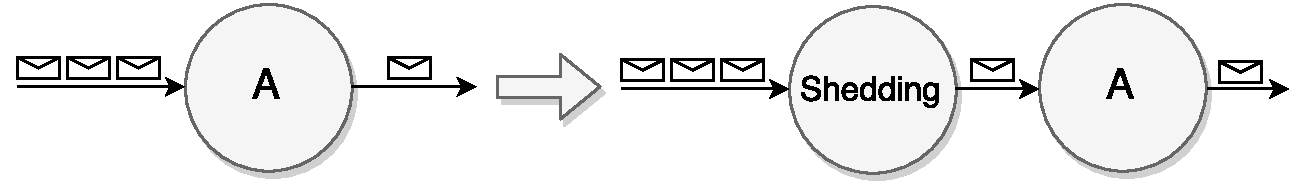
\includegraphics[scale=0.6]{images/LoadShedding.pdf}
	\caption{Load shedding en un SPS.}
	\label{fig:loadShedding}
\end{figure}

En el mundo de los SPS, varios poseen este tipo de estrategia, como por ejemplo S4 \citep{s4}, donde se establece una cota superior de eventos en cola, y en caso que su cola sea igual al límite establecido, los eventos entrantes son descartados. Otro sistema que aplica esta técnica es Aurora \citep{aurora}, el cual se basa en procesamiento de datos por ventanas de tiempo, por lo que en caso de existir una ventana de tiempo con una mayor cantidad de eventos de lo estipulado, se descarta el exceso de eventos.

Si bien esta técnica es simple y de bajo costo, siendo pensada para la disminución rápida de carga, existe una baja en la precisión y fiabilidad en los resultados. Por ejemplo, en el caso de la transferencia de video no es trascendental, dado que son pocos los pixeles perdidos, pero en una recopilación y análisis de estadísticas, esto da una menor precisión de la información obtenida por el sistema, dado que puede perderse información que estén relacionado con los comportamientos estudiados.

\subsection{Migración}
\label{sec:migracionBC}
%También se encuentra la migración, en el cual según el estado del sistema se migran los operadores de un nodo a otro. En \citep{XingZH05} se implementa   esta técnica, y si bien genera una menor carga en distintos nodos, produce un alto costo en la transferencia de los datos. Al realizar la transferencia de los datos, existe una menor tolerancia a fallos, a raíz de lo cual, se propone el uso de un búffer en el sistema, aumentando sus costos \citep{PittauACA07}.

La técnica de migración está basada en el traspaso de un operador de un nodo a otro, según el estado del sistema. En la Figura \ref{fig:migracion} se puede apreciar dos nodos, los cuales poseen tres y dos operadores respectivamente, pero debido a una sobrecarga del nodo 1 se realiza una migración de un operador al nodo 2, ya que este se encuentra con menor carga, de esta manera, se reparten homogéneamente la carga.

Si bien no existe una implementación que utilice la perspectiva según los recursos lógicos, si existe una que utiliza la perspectiva según los recursos físicos como es el caso de Borealis, el cual fue explicado anteriormente \citep{XingZH05}. Una de las principales críticas que se realiza a esta técnica, es que puede existir una falla en la comunicación del operador, donde no existe un mecanismo para evitar la pérdida de los datos. Debido a lo anterior, es que se propone el uso de \textit{buffer}, el cual tenga respaldo de la información, aumentando los costos del sistema \citep{PittauACA07}.

\begin{figure}[!ht]
	\centering
	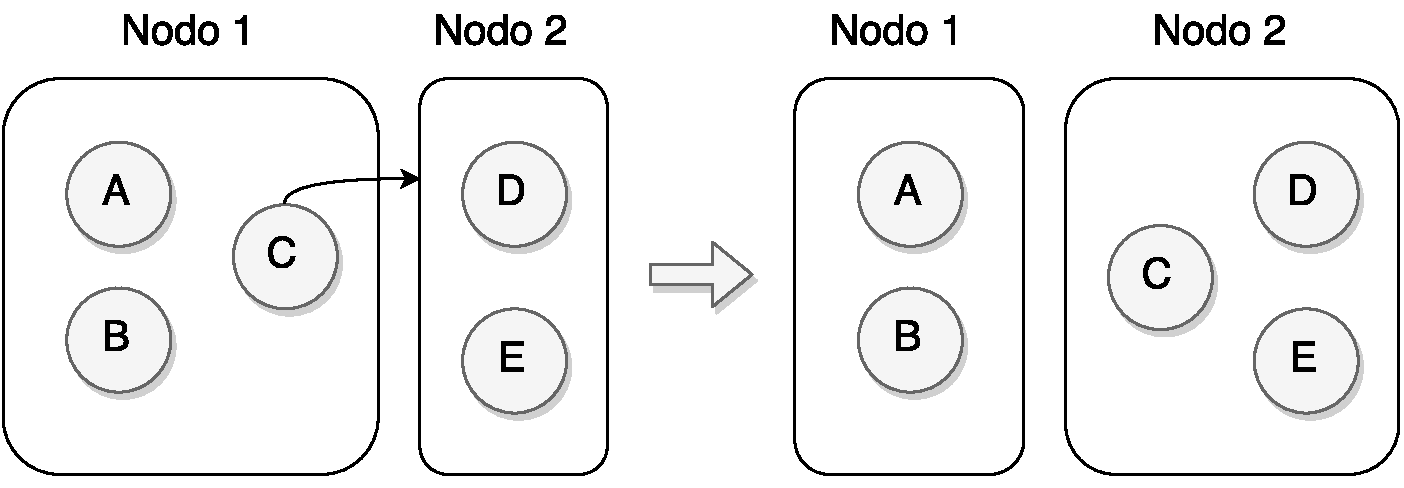
\includegraphics[scale=0.45]{images/Migracion.pdf}
	\caption{Técnica de migración en un SPS.}
	\label{fig:migracion}
\end{figure}

\subsection{Fisión}
\label{sec:fisionBC}

%Desde otra perspectiva, existen las técnicas de paralelización y replicación, las cuales se utilizan en caso de sobrepasar un umbral, el cual depende de la carga de un operador, nodo, entre otras variables. El primero consiste en paralelizar una tarea, la cual está determinada por un conjunto de operadores, en otro nodo físico \citep{IshiiS11}. En cambio, la replicación consiste en replicar un operador a nivel lógico del grafo \citep{MadsenTZ14}. Una de las características que existen en este tipo de soluciones es la elasticidad, que consiste en la capacidad de aumentar o disminuir la cantidad de operadores según la necesidad del sistema.

Otra técnica utilizada en el balance de carga es la fisión, o también llamada replicación, que permite paralelizar el procesamiento, la cual consiste en crear una réplica paralela del operador, sin perder el funcionamiento y estado. En Figura \ref{fig:fision} se presenta un operador A, el cual en primera instancia recibe un flujo de entrada $q_1$ y genera un flujo de salida $q_2$. Sin embargo, dado que este operador se sobrecarga, se procede a replicar, por lo que se hace necesario dos operadores auxiliares, en caso de poseer estado, los cuales son el operador \textit{Split} y \textit{Merge}. Estas fases son necesarias para distribuir y juntar la información respectivamente, y en general son de bajo costo. En caso de ser necesario replicar el operador \textit{Merge}, debe existir un \textit{merge} de las distintas réplicas de éste, lo cual hace más complejo el diseño del sistema, por lo que se omite su replicación.

En algunos SPS dado su funcionamiento, es que el \textit{split} y el \textit{merge} son operadores que deben ser realizados por el programador, y no de forma automática por el sistema, como S4 o Storm. Una de las características que se posee de esta técnica es que permite generar un sistema elástico, donde se puede aumentar o disminuir la cantidad de operadores según los requerimientos del sistema.

\begin{figure}[!ht]
	\centering
	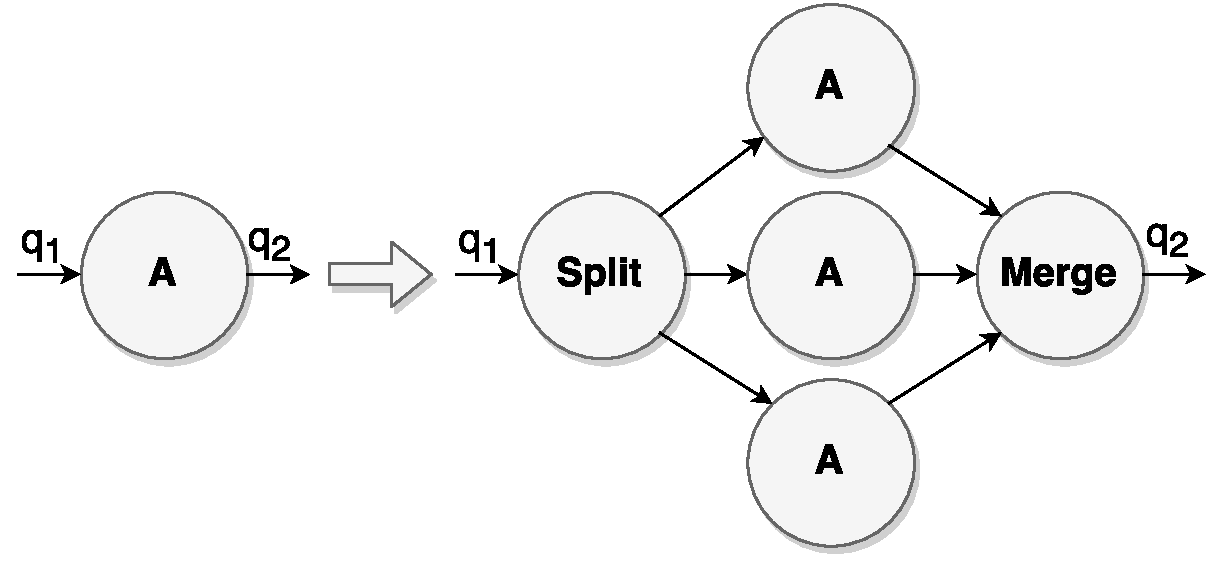
\includegraphics[scale=0.4]{images/Fision.pdf}
	\caption{Técnica de fisión en un SPS.}
	\label{fig:fision}
\end{figure}

%Una aplicación de la técnica de paralelización según el enfoque estático, es la paralelización de tareas de Storm \citep{stormtwitterdoc}, donde un conjunto de operadores realizan una tarea, indicado la cantidad de tareas que se desean ejecutar paralelamente en el sistema.

%Un ejemplo aplicado de esta técnica según el enfoque dińamico es StreamCloud \citep{GulisanoJPSV12}, que dada la cantidad de consultas que van llegando al sistema, se paralelizan las tareas existentes. Uno de los problemas que surge en estos casos son las operaciones con estado, como lo son los contadores o algoritmos de orden. La solución planteada es poseer un operador que realiza la tarea de \textit{merge}, que consiste en recibir las salidas de las tareas paralelas, agrupando los datos y proporcionando una salida según lo realizado por cada uno de las operaciones \citep{GedikSHW14}.

Una aplicación que utiliza la técnica de fisión bajo el enfoque estático, es la paralelización de tareas de Storm \citep{bookstorm}. Aquí se debe indicar en la topología del grafo la cantidad de operadores necesarios para realizar una tarea. De esta manera, por cada tarea se asigna un proceso, el cual tiene a su disposición $n$ hebras según la cantidad de operadores que se desea para cumplir dicha tarea.

Otro sistema que utiliza esta técnica, bajo un enfoque dinámico, es \textit{StreamCloud} \citep{GulisanoJPSV12}. Aquí según la cantidad de consultas realizadas al sistema se aumenta o disminuye la cantidad de operadores que cumplen las tareas que se solicitan. Para esto, es necesario un operador que distribuya los datos, denominado \textit{split}, y uno que junte la información entregadas por las réplicas del operador, denominado \textit{merge}. Por lo que este sistema sólo soporta ciertas operaciones, de tal manera que se creen de forma automática los operadores de \textit{split} y \textit{merge}. De esta manera, no existe problemas con los operadores con estado, como lo son los contadores y algoritmos de ordenamiento, dado que automáticamente realiza el procedimiento de separación y unión de los datos. Una de las características principales de este sistema, es aplicar el concepto de elasticidad, que aumenta y disminuye la cantidad de operadores según lo requerido por el sistema.

Otros trabajos como \citep{GedikSHW14, SchneiderAGBW09} también aplican este método, y paralelizan las tareas de forma elástica, y con parámetros similares, sólo que su implementación es distinta, debido que este anterior propone utilizar \textit{Cloud} para el uso del SPS. De esta manera, el enfoque se basa en la paralelización de las tareas entre las distintas máquinas.

En \citep{FernandezMKP13}, aplican fisión en el caso que exista un cuello de botella en un operador. Para la detección de estas situaciones, se posee un monitor, el cual está consultando cada cierto período de tiempo el estado de cada uno de los operadores. De esta manera, en caso que un operador sobrepase el umbral de carga establecido, el cual está determinado por la utilización de CPU se replique el operador. En la Figura \ref{fig:ejFision} se puede ver un sistema, en el cual el operador \textit{u} está enviando un flujo de datos al operador \textit{o}. Una vez \textit{o} se sobrecarga (cuello de botella), éste se debe replicar, hasta reducir la carga hasta el umbral deseado, en otras palabras, llega a la cantidad de réplicas necesarias, por lo que no es necesario seguir replicando.

\begin{figure}[!ht]
	\centering
	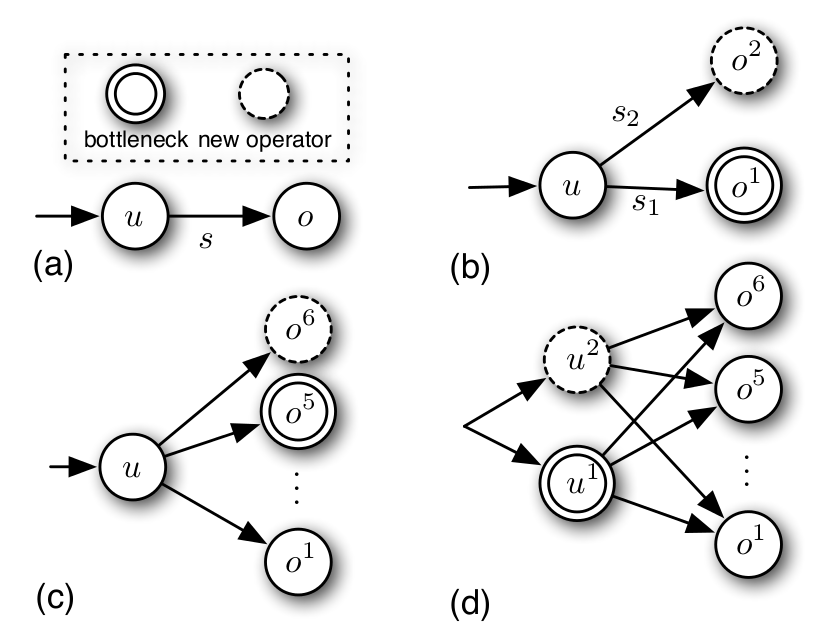
\includegraphics[scale=0.3]{images/EjFision.png}
	\caption{Ejemplo de replicación de los operadores \citep{FernandezMKP13}.}
	\label{fig:ejFision}
\end{figure}

Dentro de las desventajas existentes por parte de estos trabajos realizados, es que no utilizan la historia del operador para analizar el comportamiento a futuro de la carga. El uso de sistemas de predicción puede estabilizar el sistema cuando existen \textit{peaks} en el tráfico, debido que estos son detectados en el pasado, y se verifica si pueden ocurrir en el futuro. Otro desventaja, es que en algunos trabajos es necesario detener la ejecución de la aplicación, cambiar el número de réplicas y volver a iniciar, lo cual genera una pérdida de eventos.